\section{Вычислительные эксперименты}

\subsection{Обзор существующих датасетов}
\label{dataset}
Существует много датасетов, содержащих синтетические тексты, большинство из которых предназначено  для решения задачи бинарной классификации. Для решения задачи бинарной классификации использовался датасет 
%с текстами на английском от GPT-2\footnote{\href{https://github.com/openai/gpt-2-output-dataset.git}{GPT-2 output dataset}} и датасет 
с текстами на русском языке от различных моделей RuATD~\cite{ruatd}.

Датасетов, содержащих именно гибридные тексты не так много в силу сложности сбора таких датасетов. Большинство существующих  датасетов предназначено для решения задачи нахождения границы по предложениям. Так, первым датасетом стал Real or Fake Text~(RoFT)~\cite{dugan-etal-2020-roft} - для его создания авторы дополняли тексты с помощью моделей GPT-2. В текстах датасета сначала идет часть, написанная человеком, а далее - часть, сгенерированная языковыми моделями с помщощью человеческого префикса. Ещё один датасет, RoFT-chatgpt~\cite{kushnareva2024aigenerated}, дополняет RoFT генерациями от ChatGPT в таком же формате. Наконец, в датасете SeqXGPT~\cite{wang-etal-2023-seqxgpt} для генерации использовались открытые модели, но формат остался таким же.
Датасетов, в которых бы смена авторов была по параграфам, в открытом доступе найдено не было, поэтому для проведения экспериментов со сменой стиля по определенным позициям было решено сгенерировать свой датасет в котором бы смена авторов шла ровно по параграфам. Создание и характеристики этого датасета описаны в главе \ref{paragraphwise_split}.

\begin{figure}[h] %!t
\centering
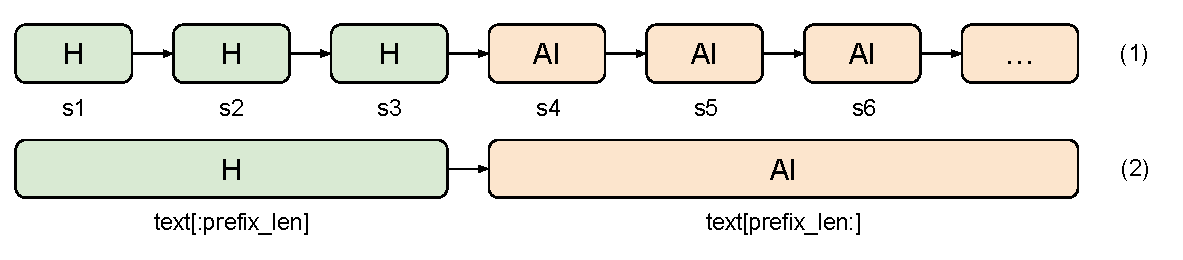
\includegraphics[width=\linewidth]{images/dataset_schemes.pdf}
\caption{Схемы авторства текстов в различных датасетах. Тег ``H'' соответствует человеческому фрагменту, ``AI'' - фрагменту, сгенерированному некотороый языковой моделью. (1) соответствует датасетам RoFT, RoFT-chatgpt и SeqXGPT, (2) - датасету SemEval2024~Task 8}
\label{schemes}
\end{figure}

Наконец, недавно было проведено несколько соревнований, в которых участникам предлагалось решить различные задачи поиска сгенерированного текста. Одним из таким соревнованием является SemEval2024~Task 8 Subtask C~\cite{semeval2024task8}, в котором предлагалось найти границу между началом, написанным человеком, и продолжением, сгенерированным с помощью языковой модели. В отличии от предыдущих датасетов, граница могла проходить в любом месте текста и по сути необходимо было решить задачу смены стиля. Датасет для соревнования был составлен с помощью моделей ChatGPT и LLaMA 2~\cite{touvron2023llama}. При этом в данном датасете встречается много текстов с некачественной генерацией~\cite{voznyuk2024deeppavlov} - например, в начале генерации модель начинает повторять человеческий префикс и это сильно упрощает задачу для детектора.

% Вторым соревнованием является DAGPap2024\footnote{\href{https://sdproc.org/2024/sharedtasks.html}{Ссылка на страницу соревнования DAGPap2024}}.Участникам предлагалось находить позиции фрагментов четырех типов - написанные человеком, сгенерированные ChatGPT, фрагменты, в которых некоторые слова были заменены на синонимы и, наконец, фрагменты, которых были суммаризированы некоторой языковой моделью. Фрагменты разного типа сменяют друг друга строго по предложениям. Однако, документы, предложенные для обучения, были очень длинными, в отличии от текстов во всех остальных датасетах. 

\begin{table}[ht]
    \centering
    \begin{tabular}{|c|c|c|}
        \hline
        Название датасета & Модели для генерации & Тип смены \\
        \hline
        RoFT & GPT-2 & по предложениям \\
        RoFT-chatgpt & GPT-2, ChatGPT & по предложениям \\
        SeqXGPT & GPT-2, GPT-Neo, GPT-J, LLaMA & по предложениям  \\
        SemEval2024 & ChatGPT, LLaMA 2 & смена стиля  \\
        % DAGPap2024 & ChatGPT &  по предложениям \\
        \hline
    \end{tabular}
    \caption{Сравнение различных датасетов для детекции фрагментов}
    \label{tab:my_label}
\end{table}

В данной работе для решения подзадач детекции фрагментов был использован датасет SemEval2024~Task 8 Subtask C.

\subsection{Описание экспериментов}

\subsubsection{Бинарная детекция}
Для решения задачи бинарной детекции сравнивалось несколько дообученных моделей на основе архитектуры BERT, некоторые из которых были мультилингвальными -  BERT,  mDeBERTa-V3, XLM-RoBERTa и ruBERT. Дополнительно было дообучены модели RoBERTa и DeBERTa.
Метрикой для сравнения была выбрана точность классификации.

\begin{table}[h!]
\centering
\begin{tabular}{|c |c |}
\hline
\textbf{Метод} & \textbf{Точность} \\
\hline
TF-IDF & 0.64223 \\
BERT-base-multilingual & 0.73430 \\
RoBERTa-base & 0.63847 \\
DeBERTa-v3-base  & 0.72661 \\
mDeBERTa-v3-base  &  0.76662 \\
XLM-RoBERTa-base & 0.72661  \\
XLM-RoBERTa-large &  0.76777 \\
ruBERT & 0.77288 \\
\hline
\end{tabular}
\caption{Точность бинарной классификации различных подходов. TF-IDF был выбран в качестве бейзлайнового решения} 
\label{tab:mae}
\end{table}

Так как датасет, на котором дообучались и оценивались модели был русскоязычным, то у моделей, которые были изначальны обучены на мультилингвальных или русскоязычных текстов, получилось более точно классифицировать тексты из тестового датасета, чем у таких же, но обученных только на английских текстах. Наилучшее качество было получено после обучения модели ruBERT - 77\%.

\subsubsection{Детекция фрагментов}
\label{paragraphwise_split}
Для бинарной сегментации мы сгенерировали набор данных из 10000 документов следующим образом: сначала мы взяли открытый датасет  со статьями с сайта Medium.com. Обрезав статьи до длины 4000 токенов, мы случайным образом выбрали до 3 абзацев, которые будут заменены на сгенерированные машиной фрагменты. Для машинной генерации мы взяли открытую модель LLaMA, так как на момент генерации это была наилучшая по качеству открытая модель. Для каждого выбранного абзаца мы давали модели предыдущий абзац в качестве промпта. 
После генерации искусственного абзаца мы обрезали его, чтобы его длина не превышала 700 токенов, и помещали его на место оригинального абзаца в документе. Наш набор данных состоит из 4000 документов с 3 замененными абзацами, 2500 документов с 4 замененными абзацами и 3500 документов с 2 замененными абзацами.

Для классификации параграфов была использована модель RoBERTa - параграфы классифицировались отдельно и их метки не зависели от меток соседних параграфов. После этого были проведены эксперименты с добавлением CRF-слоя, описанного в главе \ref{fragments}. Использование CRF позволило поднять среднюю точность классификации с 89\% до 94\%.

Дополнительно мы сравнили, как хорошо раздеялются фрагменты разного авторства. Предполагается, что взяв векторные представления двух фрагментов из одного документа разного авторства и посчитав косинусное расстояние между ними, мы получим отрицательное значение, близкое к 1, а в случае фрагментов из одного документа одного автора, косинусное расстояние должно быть положительно и близко к 1. На рис. ~\ref{sent_vs_parapgrahs} представлены результаты подсчета р
косинусных расстояний для векторный представлений соседних параграфов и соседних предложений. Видно, что параграфы хорошо разделяются, а вот предложения не так хорошо, что потверждает вывод о том, что слишком короткие тексты, например предложения, не подходят для детекции машинно-сгенерированного текста~\cite{needmoretokens, mireshghallah-etal-2024-smaller}, так детектору не хватает информации для уверенной классификации.
\begin{figure}[!htb] %!t
\centering
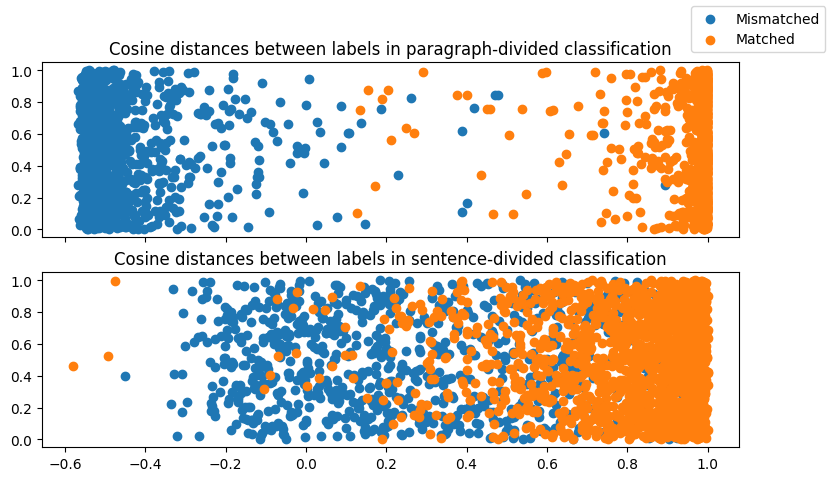
\includegraphics[width=\linewidth]{images/sent_vs_paragraphs.png}
\caption{Расстояния между векторными представлениями фрагментов разного авторства в случае, если а) фрагментами являются параграфы б) фрагментами являются предложения}
\label{sent_vs_parapgrahs}
\end{figure}




\subsubsection{Детекция смены стиля}

Датасет SemEval2024~Task 8 Subtask C оказался достаточно маленьким, поэтому для получения обучающей выборки достаточно большого размера и для внесения большего разнообразия в положении индекса смены авторов предварительно была сделана аугментация данных. До аугментации данных в обучающей выборке было 3648 текстов, после аугментации получилось 8059 текстов.


На рис. \ref{statistics} показаны две основные статистики текстов в исходных датасетах, которые были полезны для решения - длины текстов и положение индекса смены авторов. Почти все тексты в обучающей и тестовой выборке были достаточно короткими - до 1000 токенов. Видно, что в большинстве текстов смена авторов происходит в окне с 0 по 400 токен, поэтому для токенизатора даде окна в 512 токенов было достаточно и на таком размере окна результаты получились даже лучше, чем на более длинном окне. 

 \begin{figure*}[!htb]
    \centering
    \subfloat[Распределение длин текстов]{%
        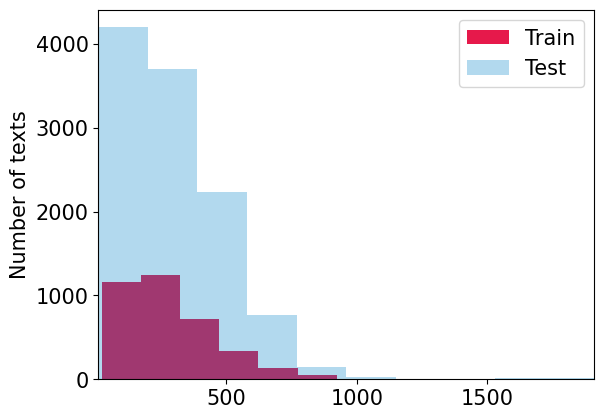
\includegraphics[width=0.5\linewidth]{images/plot_lengths.png}%
        \label{fig:a}%
        }
    \hfill%
    \subfloat[Положение индекса смены стиля]{%
        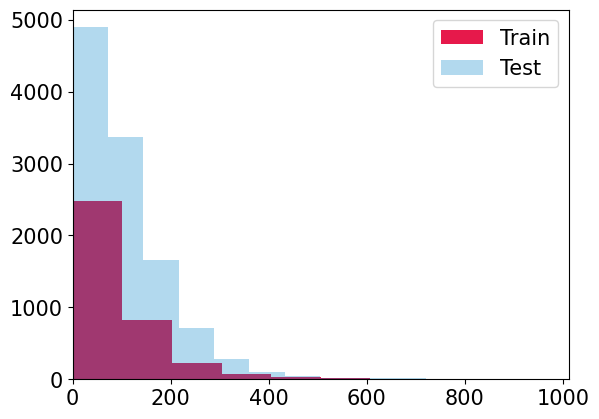
\includegraphics[width=0.5\linewidth]{images/plot_subtokens.png}%
        \label{fig:b}%
    }
    \caption{Статистики текстов в датасете после токенизации}
    \label{statistics}
\end{figure*}

Все эксперименты были проведены на двух наборах данных - на исходных данных от организаторов и на аугментированных данных. Сравнивались три модели: Longformer,  RoBERTa и DeBERTaV3. Организаторы соревнования предлагали использовать Longformer-base в качестве базового решения. Результаты экспериментов представлены в таблице \ref{tab:mae}. Из данных экспериментов можно сделать следующий вывод: даже простая аугментация данных позволяет довольно сильно улучшить результаты работы метода. Использование DeBERTaV3-large позволило довольно сильно улучшить не только решение организторов, но и лучшее решение с соревнования.
\begin{table}[ht!]
\centering
\begin{tabular}{|c |c | c |}
\hline
\textbf{Модель} & \textbf{Исходный датасет} & \textbf{Новый датасет} \\
\hline
RoBERTa-base &  31.56  & 30.71\\
RoBERTa-large & 25.25 &20.66\\
\hline
longformer-base  &  23.16 &22.94 \\
longformer-large  &  22.97 &20.33 \\
\hline
DeBERTaV3-base & 16.12 &13.98 \\
DeBERTaV3-large &  15.16 &\textbf{13.38} \\
\hline
Top~1 соревнования & 15.68 & - \\
\hline
\end{tabular}
\caption{Метрика MAE на исходных и новых (аугментированных) данных. Дополнительно приведено лучшее решение, получившее первое место по результатам соревнования} 
\label{tab:mae}
\end{table}